\section{Comparison of emissivity models in the CRTM}
%====================================================

The microwave sea surface emissivity model use dint eh current CRTM release (v1.1) is Fastem1\cite{Fastem1}. Comparison of this model with the updated LF\_MWSSEM model, as well as with Fastem3 (REF!), for the low frequency ($f\!>$20GHz) channels of the Aqua AMSR-E instrument are shown in figure \ref{fig:AMSR-E_Model_Comparison}. The difference between the Fastem1 and new models is very large for the lowest frequency with a $\sim$20\% decrease in teh computed emissivity at 6.925GHz. The percentage change decreases as the frequency increases with a more modest $\sim$5\% decrease at 18.7GHz. The difference between the LF\_MWSSEM and Fastem3 models is relatively uniform at $\sim$2-5\% for all frequencies.

\begin{figure}[htp]
  \centering
  \begin{tabular}{c}
    \textsf{(a) Model emissivities for low frequency AMSR-E channels}\\
    \includegraphics[bb=85 411 540 556,clip,scale=0.8]{graphics/Comparison/AMSR-E_Model_Comparison.eps}\\
    \textsf{(b) Model emissivity comparisons with Fastem1 for low frequency AMSR-E channels}\\
    \includegraphics[bb=85 225 540 380,clip,scale=0.8]{graphics/Comparison/AMSR-E_Model_Comparison.eps}
  \end{tabular}
  \caption{Comparison of different emissivity models for the low frequency AMSR-E channels. \textbf{(a)} The computed emissivity spectra. Note the large difference between Fastem1 (current CRTM model) and the other models. \textbf{(b)} The emissivity spectra differences with respect to Fastem1. The newer models provide a 20\% decrease in the computed emissivties at these frequencies.}
  \label{fig:AMSR-E_Model_Comparison}
\end{figure}

The impact of these emissivity model changes on computed brightness temperatures was gauged by running the standard CRTM ``smoke test''\footnote{a simple test to catch large defects but disregard trivial ones.} using a small set of climatological profiles for a series of microwave instruments: Aqua AMSR-E, NOAA-18 AMSU-A and MHS, and DMSP-16 SSMIS. The average and RMS brightness temperature difference for the LF\_MWSSEM-Fastem1 test runs are shown in figure \ref{fig:LF_MWSSEM-Fastem1.TBstats}. As expected, for the lowest frequencies of AMSR-E the temperatures differences are very large at $\sim$30K. For the other instrument where the frequencies of the surface sensitive channels are generally greater than 20GHz, the differences are smaller, but still significant in the 1-5K range.

\begin{figure}[htp]
  \centering
  \begin{tabular}{c}
    \textsf{(a) Aqua AMSR-E LF\_MWSSEM-Fastem1 CRTM test statistics}\\
    \includegraphics[bb=85 225 540 380,clip,scale=0.8]{graphics/Comparison/amsre_aqua.TBstats.eps}\\
    \textsf{(b) NOAA-18 AMSU-A LF\_MWSSEM-Fastem1 CRTM test statistics}\\
    \includegraphics[bb=85 225 540 380,clip,scale=0.8]{graphics/Comparison/amsua_n18.TBstats.eps}\\
    \textsf{(c) NOAA-18 MHS LF\_MWSSEM-Fastem1 CRTM test statistics}\\
    \includegraphics[bb=85 225 540 380,clip,scale=0.8]{graphics/Comparison/mhs_n18.TBstats.eps}\\
    \textsf{(d) DMSP-16 LF\_MWSSEM-Fastem1 CRTM test statistics}\\
    \includegraphics[bb=85 225 540 380,clip,scale=0.8]{graphics/Comparison/ssmis_f16.TBstats.eps}
  \end{tabular}
  \caption{CRTM $\Delta T_B$ statistics between the LF\_MWSSEM and Fastem1 models. \textbf{(a)} Aqua AMSR-E. Note that beyond channel 6, $f\!>$20GHz so the LF\_MWSSEM invokes Fastem3. \textbf{(b)} NOAA-18 AMSU-A. All AMSU-A channels are $f\!>$20GHz. \textbf{(c)} NOAA-18 MHS. Again, all MHS channels are $f\!>$20GHz. \textbf{(d)} DMSP-16 SSMIS.}
  \label{fig:LF_MWSSEM-Fastem1.TBstats}
\end{figure}

For comparison, the average and RMS brightness temperature difference for the LF\_MWSSEM-Fastem3 test runs are shown in figure \ref{fig:LF_MWSSEM-Fastem3.TBstats}. Only for those channels with frequencies less than 20GHz show any impact but the differences are still quite large. Note that the SSMIS channels are not ordered in increasing frequency, hence the $\Delta T_B$ spikes for channel 12 and 13 ($f\!=$19.35GHz)

\begin{figure}[htp]
  \centering
  \begin{tabular}{c}
    \textsf{(a) Aqua AMSR-E LF\_MWSSEM-Fastem3 CRTM test statistics}\\
    \includegraphics[bb=85 401 540 556,clip,scale=0.8]{graphics/Comparison/amsre_aqua.TBstats.eps}\\
    \textsf{(b) NOAA-18 AMSU-A LF\_MWSSEM-Fastem3 CRTM test statistics}\\
    \includegraphics[bb=85 401 540 556,clip,scale=0.8]{graphics/Comparison/amsua_n18.TBstats.eps}\\
    \textsf{(c) NOAA-18 MHS LF\_MWSSEM-Fastem3 CRTM test statistics}\\
    \includegraphics[bb=85 401 540 556,clip,scale=0.8]{graphics/Comparison/mhs_n18.TBstats.eps}\\
    \textsf{(d) DMSP-16 LF\_MWSSEM-Fastem3 CRTM test statistics}\\
    \includegraphics[bb=85 401 540 556,clip,scale=0.8]{graphics/Comparison/ssmis_f16.TBstats.eps}
  \end{tabular}
  \caption{CRTM $\Delta T_B$ statistics between the LF\_MWSSEM and Fastem3 models. Where the LF\_MWSSEM invokes Fastem3 (for $f\!>$20GHz), the differences are identically zero. \textbf{(a)} Aqua AMSR-E. \textbf{(b)} NOAA-18 AMSU-A. \textbf{(c)} NOAA-18 MHS. \textbf{(d)} DMSP-16 SSMIS. Channels 12 and 13 have $f$=19.35GHz.}
  \label{fig:LF_MWSSEM-Fastem3.TBstats}
\end{figure}


